% Motivation model diagram Heckhausen and Rheinberg
% Author: Stefan Kottwitz
\documentclass{article}
%%%<
\usepackage{verbatim}
%%%>
\usepackage{tikz}

\begin{document}
  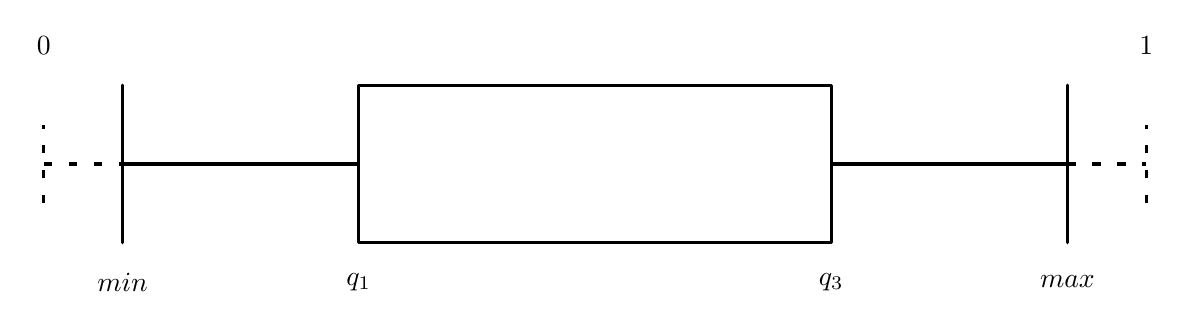
\begin{tikzpicture}[very thick]
    \node at (0,3.5) {0};
    \draw [loosely dashed] (0,1.5)  --     (0,2.5);
    \draw [loosely dashed] (0,2)    --     (1,2);
    \draw [cap=round]      (1,1)    --     (1,3);
    \node at (1,0.5) {$min$};
    \draw                  (1,2)    --     (4,2);
    \node at (4,0.5) {$q_1$};
    \draw [join=round]     (4,3) rectangle (10,1);
    \node at (10,0.5) {$q_3$};
    \draw                  (10,2)   --     (13,2);
    \draw [cap=round]      (13,1)   --     (13,3);
    \node at (13,0.5) {$max$};
    \draw [loosely dashed] (14,1.5) --     (14,2.5);
    \draw [loosely dashed] (13,2)   --     (14,2);
    \node at (14,3.5) {1};
  \end{tikzpicture}

\end{document}
